
%(BEGIN_QUESTION)
% Copyright 2007, Tony R. Kuphaldt, released under the Creative Commons Attribution License (v 1.0)
% This means you may do almost anything with this work of mine, so long as you give me proper credit

En forbedring i forhold til endebrytere med fysisk kontakt kan i mange tilfeller være kapasitive nærhetssensorer. Denne type bryter aktiveres ved at et objekt kommer nærme den. Det er ikke nødvendig med fysisk kontakt. Forklar hvordan denne type bryter virker, og hvilke materialer den kan detektere. 

kapasitive nærhetssensorer trenger driftsspenning. Det er vanlig med +24V DC. Utgangen er normalt ikke en potensialfri kontakt, men en transistor. 

$$\includegraphics[width=15.5cm]{i02244x01.eps}$$

\vskip 30pt

Vis hvordan du ville koblet kretsen nedenfor slik at LED-en lyser når sensoren aktiveres. Anta at utgangen er sinking (NPN). 

\vskip 20pt \vbox{\hrule \hbox{\strut \vrule{} {\bf Suggestions for Socratic discussion} \vrule} \hrule}

\begin{itemize}
\item{} Identify an object an inductive proximity switch would be able to detect.
\item{} Identify an object an optical proximity switch would be able to detect.
\item{} Identify an object a capacitive proximity switch would {\it not} be able to detect.
\item{} Identify an object an ultrasonic proximity switch would {\it not} be able to detect.
\end{itemize}

\underbar{file i02244}
%(END_QUESTION)





%(BEGIN_ANSWER)


%(END_ANSWER)





%(BEGIN_NOTES)

$$\includegraphics[width=15.5cm]{i02244x02.eps}$$

%INDEX% Switch, proximity: inductive

%(END_NOTES)


